\chapter{Introduction}
\label{chapter:Introduction}


\section{Motivation}
\label{sec:motivation}

In the past decade, deep neural networks have been responsible for several breakthroughs in machine learning, ranging from computer vision to natural language processing~\cite{Goodfellow-et-al-2016}. These astounding achievements suggest that deep neural networks have the potential to lead to many more groundbreaking applications of machine learning. However, a closer look at these breakthroughs reveals that most of the applications focus on one of two kinds of data: images and natural language. An image (in the most general sense) can be described as data-points (pixels) on a two-dimensional grid. Natural language on the other hand has a purely one-dimensional structure. In text-form, it can be described as a sequence of words, syllables or characters. In the form of speech, it is a sequence of sounds. In either case, the structure of the data is purely sequential, meaning that each data point (e.g. a word or a character) is fully described by its position in the 1D sequence.

Two classes of deep neural architectures were responsible for the breakthroughs: convolutional neural networks (CNNs) for computer vision and recurrent neural networks (RNNs) for natural language~\cite{Goodfellow-et-al-2016}. Both model classes have seen tremendous improvements over these last years, but all of them are built on the same basic architectures~\footnote{Recently, \textit{Transformer}-architectures~\cite{Vaswani2017} have largely replaced RNN-based architectures in natural language processing. Up until this point, advanced RNN-architectures, such as \textit{Long Short Term Memory networks} (LSTMs)~\cite{Hochreiter1997} have been responsible for the advances in the field.}. For this reason, the basic strategy in applied deep learning can be over-simplified as: Use the latest convolutional architecture that suits the task at hand in computer vision and use the latest RNN-based (e.g. LSTM) or Transformer architecture in natural language processing.

However, if the data for the use-case at hand does not fit into either of those two categories, the situation is much more complicated. In other areas, deep neural networks have not outperformed traditional methods by as large a margin and the choice of approach is not as obvious. Examples include documents that comprise both, text and visual elements, such as invoices, legal documents, etc. These documents cannot be fully described as a text-sequence because the position of words, amounts or dates on the page strongly affects their interpretation. (In contrast to pure text, such as a novel, where a word's meaning obviously depends only on the words before and after in the 1D sequence of words and not on its position on the page.) However, they also cannot be treated merely as images as the textual information is vital. Thus, they represent textual information on a 2D grid for which there is no go-to deep learning architecture yet~\footnote{
	An interesting approach to combine convolutional networks with textual information is the so-called chargrid~\cite{Katti2020}. In short, each pixel on the image is mapped to character (including a 'null-character'). These characters are then represented as channels in the input to the convolutional network. Just like a regular image has three color channels, a chargrid with n characters has n-input channels. The same concept can be expanded to words or syllables as well. While the results are promising, this model-class does not outperform more traditional machine learning models with manual feature engineering (e.g. decision tree-based models) by a large margin. A similar breakthrough as in computer vision where all previous techniques have been made obsolete by the invention of CNNs has therefore not yet been achieved for 2D documents.
}. Another example is 3D data, such as point-clouds~\cite{Charles2017} or molecular structures. In theory, CNNs can be extended to three or higher dimensions, but in practice this approach is computationally not feasible due to the cubic number of data points in three dimensions.

From these considerations, it becomes clear that it is not trivial to extend the success of DNNs from images and language to other kinds of data. Nevertheless, the potential for progress is tremendous and warrants research into neural networks for other kinds of data.

One of the most-versatile data structures is the graph. A graph contains a set of data points called vertices or nodes and a set of edges that define relations between the nodes. As such, a graph is inherently unordered and thus suited for modeling data without predefined order. The only kind of structure that has to be imposed is the definition of the edges. Thus, the only kind of inductive bias of a graph are the relations between nodes~\cite{Battaglia2018}. This relational inductive bias is a rather weak bias and allows many kinds of data to be modeled as a graph without imposing some kind of structure onto the data that is not there.

The class of neural networks for graph structured data are called Graph Convolutional Networks (GCNs)~\cite{Kipf2017}~\cite{Schutt2017} or Message Passing Neural Networks (MPNNs)~\cite{Gilmer2017}. The terminology is different between GCNs and MPNNs, but the underlying principles are the same and most neural network architectures for graphs can be described in either framework. While the MPNN terminology is somewhat more intuitive to understand, the graph convolution terminology has the advantage of highlighting the parallels to regular CNNs. In this thesis, we will mostly adhere to the more common message passing terminology, but also borrow terms from the graph convolution terminology to highlight the parallels with and differences from regular CNNs.

Obvious applications of MPNNs are molecular structures (the topic of this thesis) and social media networks (or any system where users / people interact with each other)~\cite{Zhou2018}. Moreover, many kinds of data that do not seem to have an obvious graph structure at first sight can be modeled as graphs and thus analyzed with MPNNs as well. Examples include 3D point clouds~\cite{Charles2017} or invoices (with words as nodes and the spacial relationship between words as edges)~\cite{Riba2019}.

In the remainder of this section we will mostly refer to molecular structures as examples of graph structured data, but keep in mind that most principles apply to other kinds of graphs as well. In particular, the most important challenge when modeling molecular structures as graphs is the loss of some of the 3D structural information, as discussed in Section~\ref{sec:lack-of-3d-structure}. This challenge is exactly the same for any other 3D data represented as a graph.

\section{Message Passing Neural Networks}

In this section we will review Message Passing Neural Networks (MPNNs) in general. While all those considerations also apply when the input graphs represent molecules, Section~\ref{3d-molecules-for-gcnns} will show the specific challenges for this use case.

\subsection{Challenges of graph structured data for deep neural networks}
\label{sec:graph-challenges}

There are several challenges when designing neural networks for graphs.

\paragraph{No fix-sized dimension (globally)}
Each graph can have a different dimension in terms of number of nodes and edges. This, per se, is nothing graph-specific. After all, images also come in different sizes. However, while images can be cropped and scaled to have the same dimension if needed, there is no easy way to do something equivalent with graphs. For instance, in a dataset of 3D molecular structures, the molecules typically have different numbers of atoms (nodes) and there is no reasonable way to change this.
\paragraph{No fix-sized dimension (locally)}
In a regular graph (without isolated nodes), a node can have 1 to n neighbor-nodes. This has important implications for constructing a graph convolution operation because it requires a function that is invariant to the number of nodes in the neighborhood. We cannot just define a fixed-sized kernel function and apply it to parts of the graph analogous to regular CNNs.
\paragraph{No inherent order of nodes}
In a graph, there is no inherent order of nodes. We cannot define a first node, second node, etc. and compare those across graphs (for comparison, note that this is possible in images as every image has an upper left corner, a center, etc.). The same reasoning applies to the neighborhood of any one node: there is no unambiguous way of ordering the neighbor-nodes that allows them to be compared to the neighborhood of another node. Again, this has important implications for graph convolution because it requires a function that is invariant to the order of the nodes.

From the last two paragraphs, one can already suspect that any neural network for graph structured data will require some sort of aggregation function, such as \textit{mean}, \textit{sum} or  \textit{max}. These functions work with a varying number of input nodes and are invariant to their order (permutation invariant).

Now that we briefly described the properties of the input data, we will examine the possible output formats of a MPNN in the next section. With the input data and the output defined, we will then focus on the transformations that map the input to the output in MPNNs.

\subsection{Output format of Message Passing Neural Networks}
\label{sec:graph-output}

MPNNs can be used to predict three kinds of target variables.

\paragraph{Graph-properties}
The target variable is a scalar or vector per graph. For instance, this could be properties of a molecule to be predicted from its 3D structure. This is the only type of output format where the output-dimension is constant across graphs, even though the graphs themselves have different dimensions.
\paragraph{Node-properties}
The target variable is some property of a single node. Thus, for each node in the graph, a scalar or vector has to be predicted. In the example of molecular structures, this would be a property of individual atoms.
\paragraph{Edge-properties}
In this case, the target variable is a scalar or vector-valued edge-property, i.e. a property of the interaction between two nodes. In molecules, an edge-property could for instance be the interaction energy between two atoms.

Note that for the second two types of target variables, the output dimension depends on the dimension of the input graph, while only the graph-properties as target variables produce output with a constant dimension akin to a regular CNN.

\subsection{Components of Message Passing Neural Networks}


The basic building block of a MPNN is a so called message passing step that maps a given node-representation and the neighborhood of the node to an updated node representation. This step can also be called  graph convolution layer, as it shares some commonalities with regular convolution layers. Here, we will use the message passing terminology suggested by Gilmer et al.~\cite{Gilmer2017} to describe this step, but refer to it as graph convolution occasionally to highlight the analogy to regular CNNs.

The input data can be described as a graph $G$ with	a set of node features and (optionally) a set of edge features. The features of a given node $v$ are denoted as $x_v$, while $e_{vw}$ describes the features of the edge between node $v$ and node $w$. For simplicity, we will assume undirected graphs where $e_{vw}$ is equal to $e_{wv}$, which is reasonable for modeling 3D structural data. However, directed graphs can be described in the same framework if the application requires directed edges. Finally, let $T$ be the number of graph convolutional layers or the number of message passing steps and denote a specific step as $t \in \{1, 2, ..., T\}$. Furthermore, the node representation at any hidden layer $t$ shall be denoted as $h_v^t$. Note that compared to an image in regular CNNs, the node features $x$ are equivalent to the image, while the hidden node representations (also called hidden states) $h$ are equivalent to the feature maps after the first convolutional layer.

During each message passing step, the hidden representation of each node $h_v^t$ is updated to $h_v^{t+1}$ using the following procedure:

\begin{equation}\label{eq:message-function}
m_v^{t+1} ~=~ \sum_{w \in N(v)} M_t(~h_v^t,~ h_w^t,~ e_{vw}~)
\end{equation}

\begin{equation}\label{eq:update-function}
h_v^{t+1} ~=~ U_t(~h_v^t, ~m_v^{t+1}~)
\end{equation}


The above two steps are comprised of three functions:

\begin{enumerate}
	\item The message function $M$ computes the 'message' from node $w$ to node $v$ using the hidden representations of both nodes as well as the features of the connecting edge. A specific architecture may not use all the arguments of the message function in the general framework. For instance, the message function may not use the receiving node hidden state $h_v^t$ (which is used in the next step anyway) or the edge features. In the simplest case, the message function could just be a concatenation of the arguments, such as $m_v^{t+1} = (h_w, e_{vw})$~\cite{Duvenaud2015}. A more complex message function could be a multilayer perceptron (MLP), which takes the concatenation $(h_v, h_w, e_{vw})$ as input~\cite{Battaglia2016}.
	
	\item An aggregation function aggregates the messages from all the neighboring nodes of node $v$. Any function that is permutation invariant and works for any number of nodes, such as $sum$, $mean$, $min$ or $max$, can be used at this step. However, in practice, the reasonable options are mostly limited to summation and the arithmetic mean.	
	In other papers, aggregation is described as a separate step and the aggregation function denoted with a specific symbol. Here, as well as in Gilmer et al.~\cite{Gilmer2017}, we simply use the summation (Equation~\ref{eq:message-function}) and note that it could be replaced by the arithmetic mean if appropriate.
	The aggregation is not a function with learned parameters and has to be chosen by the architect of the MPNN. Moreover, it can lead to considerable loss of information. However, this step is inevitable because the neighborhood of a given node can consist of any number of nodes and they do not have an inherent order, as discussed in Section~\ref{sec:graph-challenges}.
	
	\item The update function $U$ (Equation~\ref{eq:update-function}) updates the hidden state $h^t$ based on  $m_v^{t+1}$, the aggregated messages from its neighboring nodes. Examples of update functions include for instance $h_v^{t+1} = \sigma(H_t^{deg(v)} m_v^{t+1})$, which essentially corresponds to passing the message for node $v$ through a 'one-layer neural network' while having a separate network for each message passing step $t$ and each node degree $deg(v)$~\cite{Duvenaud2015}~\footnote{
		Of course, this definition only makes sense in graphs where the maximum node degree is a reasonably low number  and varies from node to node. In most experiments in this thesis (Section~\ref{sec:alchemy}), complete graphs are used where each node has the same degree (the number of nodes in the graph), such that $deg(v) =|G|~~ \forall~ v \in G$. For such a setting, this definition of the update function would of course not be applicable.
	}. Another example of an update function is an MLP, which takes the concatenation $(h_v, x_v, m_v)$ as input~\cite{Battaglia2016}.
\end{enumerate}

Apart from these essential components of the message passing framework, an edge-update function can be added as an optional step. This function updates the edge-representation at each message passing step analogous to the node update function defined in Equation~\ref{eq:update-function}. The edge update function can be defined as $e_{vw}^{t+1} ~=~ E(h_v,~ h_w,~ e_{vw}^{t})$, where $E$ can be defined in many different ways just like the node update function~\cite{Kearnes2016}~\cite{Jørgensen2018}. However, edge-updates are not frequently used in the MPNNs.

Finally, if the target variable is a property of the whole graph, a readout function is required to map the node representations to the target.

\begin{equation}\label{eq:readout-function}
	\hat{y} ~=~ R~(~\{~h_v^T\ ~|~ v \in G~\}~)
\end{equation}


Because the readout function is a function of all nodes in the graph, it has to handle varying numbers of nodes and be permutation invariant. Thus, just like the message function defined in Equation~\ref{eq:message-function}, it has to include some sort of aggregation, such as \textit{sum} or \textit{mean}. This aggregation could occur as the very last step, such as in Schütt et al., where all hidden node representations are passed separately through an MLP and then summed up~\cite{Schutt2017}. In contrast, in Chen et al., the final step of the readout function is an MLP, which takes the already aggregated node representations as input~\cite{Chen2019}.

In most architectures, the weights of both functions are shared, such that $M_t$ and $U_t$ are the same for all message passing steps $t$. However, this is not a necessity and one can also build a MPNN with different weights for each message passing step. Section~\ref{sec:weight-sharing} presents an experiment comparing the two approaches.

In the first message passing step, only first degree neighbor nodes have an impact on the updated node hidden states. In the second step, second degree neighbors have an indirect impact, as they already influenced the hidden state of the first degree neighbors in the previous step. Thus, at each step $t$, $h_v^t$ is influenced by nodes with a path length of at most $t$ edges apart from node $v$. If the number of steps $T$ is sufficiently large, eventually, the whole graph might have an indirect influence on the hidden state $h_v^T$. However, the first degree neighbors will always have the most direct influence, followed by the second degree neighbors, etc.

With a block of $T$ message passing steps, one has successfully constructed a mapping to create higher-level features akin to the convolutional layers of a regular CNN. Now, we can examine how these higher-level features can be mapped to the desired output. While the message passing part of the MPNN can be the same for each of the three types of output format discussed in Section~\ref{sec:graph-output}, the head of the MPNN needs to be tailored depending on the desired output format.

\begin{enumerate}
	\item \textbf{Graph properties}. To predict graph properties, the higher-level node features computed by the convolutional layers have to be mapped to the target variable using a readout function $R$ defined in Equation~\ref{eq:readout-function}. Again, due to the variable number of nodes and the lack of any inherent order, this requires an aggregation function, which is permutation invariant and works for different numbers of nodes. Similarly to aggregation during message passing, summation and the arithmetic mean are typically the only viable options.
	Just as during message passing, the aggregation step in the readout function potentially looses valuable information. However, due to the inherent challenges of graph structured data (Section~\ref{sec:graph-challenges}), it is difficult to find a better solution. As the nodes can be regarded as an unordered set, \textit{Set2Set}~\cite{Vinyals2015} and similar methods can be used in the readout function.
	\item \textbf{Node properties}. In this simple case, the readout requires only a mapping from the final node hidden state $h_T$ to the output variable, which can again be achieved with a shallow MLP.
	\item \textbf{Edge properties}. To predict edge properties, a readout function needs to take the two connected node's hidden states (and optionally also the edge features) as input and map it to the desired output.~\footnote{Some architectures use edge-updates analogous to update of node representation in regular MPNNs~\cite{Jørgensen2018}. In this case, a mapping from the final hidden state to the desired output format can suffice as a readout function - equivalent to how node properties are predicted.}
\end{enumerate}


In summary, a MPNN is composed of two parts: message passing (graph convolution) and readout function. The framework introduced here allows to describe highly different architectures using the same terminology. In Section~\ref{sec:mpnn-architecture}, the basic architecture of a MPNN used in this thesis is described in detail.

\section{Predicting molecular properties from 3D structure with Message Passing Neural Networks}
\label{3d-molecules-for-gcnns}

\subsection{Deep neural networks in chemical applications}

3D structures of small chemical compounds as well as large biomolecules are readily available on a large scale~\cite{Ruddigkeit2012}~\cite{Chen2019}~\cite{Ramakrishnan2014}.
However, just knowing the 3D structure of a molecule does not go a long way towards understanding its biological function (in the case of biomolecules) or its molecular properties and potential applications (in the case of of small organic molecules). For instance, in drug discovery, a huge amount of effort goes into laborious and costly experiments on a large scale to find the right small organic molecule for the right therapeutic target~\cite{Fda-drug-discovery}. Speeding up and improving this process is highly desirable for obvious reasons. 
One way to address this issue is to create purely computational experiments. In the life science context, these experiments are often referred to as in-silico analogous to in-vitro (in a test-tube) and in in-vivo (in a living organism).

%Such in in-silico experiments can be created with molecular structures using molecular dynamics simulations (MDS). In short, MDS creates artificial force-fields to simulate real physical forces to simulated the behavior of molecules under certain conditions~\cite{Hospital2015}. Large biomolecules are usually modeled down to the level of atoms while small molecules are modeled down to the level of subatomic particles (electrons, protons, etc.). MDS is extremely valuable not only as a proxy for in-vitro experiment but also for understanding the underlying dynamics that produce the experiments outcome. However, it is also extremely challenging to mimic realistic experimental conditions: it requires an enormous amount of expertise in life science and chemistry, strong computational skills and extensive experience with MDS itself. Furthermore, MDS is also computationally very expensive and thus cannot be used as a cheap proxy for in-vitro experiments at a large scale.



% dnns have the potential to extract valuable information from 3D structures using vast amounts of data with ground-truth without having to explicitly model the underlying physical forces and the interplay of subatomic particles.

\subsection{Representing molecules as graphs}
\label{sec:molecules-as-graphs}

Figure~\ref{fig:molecule-3d} shows an illustration of a 3D molecule structure. The raw data contains only coordinates and atom types. The presence or absence of bonds between atoms can be derived from the types of atoms and the distance between them. Thus, the raw data of a molecule is only an unordered set of tuples of the form $(a, \vec{c})$
with $\vec{c} \in \mathbb{R}^3$ being the coordinate vector
and $a \in \{1, 2, ... N_a\} $ representing the atom type with $N_a$ being the number of atom-types in the dataset - which is seven in the dataset at hand~\footnote{
	Hydrogen (H), carbon (C), nitrogen (N), oxygen (O), fluoride (F), sulfur (S) and chlorine (Cl)
}. The cardinality of the set is the number of atoms in the molecule and varies from molecule to molecule.

\begin{figure}[H]
	\centering
	\includegraphics[width=\linewidth]{figures/molecule-3d-1}
	\caption{A 3D structure of a small organic molecule. Carbon and hydrogen atoms are shown in gray and white, respectively. The red spheres show oxygen atoms and the blue one shows a nitrogen atom, according to the common coloring convention. The size of the spheres is chosen such that covalently bonded atoms have no or almost no space between them.
}
	\label{fig:molecule-3d}
\end{figure}

When it comes to 3D structures, there are really only two basic ways of representing them for neural networks. The first is to describe them as 3D grids and to use 3D convolutional networks simply extending the same architectures used in computer vision by an additional dimension~\cite{Wallach2015}. In this approach, you would literally use the 3D color image shown in Figure~\ref{fig:molecule-3d} as model input. The problem with this approach is two-fold: First of all, the cubic number of data-points makes this method computationally very expensive. The second problem is that the information encoded in all these data-points is highly redundant. In molecular structures, coordinates and types of atoms are fully sufficient to describe the molecule. All other information - such as atomic radius, etc. - are functions of the types of atoms (hydrogen, carbon, etc.). Thus, when, for instance, a ten-atom molecule is fully described by ten coordinate vectors and ten atom types (40 numbers), it is excessive and inefficient to model it as a 3D image with tens or hundreds of thousands of pixels. The advantage of the 3D convolutional approach is that 3D structure information is provided to the model, which is a challenge for MPNNs, as explained in the next section.


The second approach of representing molecules for neural networks is to use graphs. The idea of using graphs to model molecules comes quite naturally when looking at the most common way of representing small molecules in text books: so called molecule graphs, such as the one shown in Figure~\ref{fig:caffeine}. A molecule is usually defined as a number of atoms connected by covalent bonds. These kind of bonds involve the sharing of one or more electron-pairs between the bonded atoms and are chemically very stable - it takes considerable energy or enzymes to break them up~\cite{Organic-chemistry}. In laymen's terms, covalent bonds can be regarded as 'stable under normal conditions'. In the commonly used molecule graph representation, atoms are shown as letters denoting their type and the covalent bonds are drawn as edges between them, as shown in Figure~\ref{fig:caffeine}. Thus, defining a graph where atoms are the nodes and covalent bonds are the edges seems like the most natural way of modeling molecules. However, upon closer examination, the situation is somewhat more complicated.

Atoms interact not only if they are covalently bonded. There is a wide array of non-covalent interactions that have a large influence on molecular properties, such as Van der Waals forces (a simple example being positive and negative partial charges)~\cite{Organic-chemistry}. The strength of non-covalent interactions is a function of atom types, distance and the local environment in the 3D structure. Thus, only including covalent bonds leads to considerable loss of information. For instance, two atoms can be close in space and interact non-covalently, even though the path length in the covalent graph may be quite large.

With these considerations, another way of representing a molecule as graph is to simply define an edge between every pair of atoms if the distance between them is below a certain threshold. Yet another way of constructing the graph is to draw an edge between any given atom and it's k nearest neighbors.


\begin{figure}[H]
	\centering
	\includegraphics[width=0.6\linewidth]{figures/caffeine}
	\caption{The standard molecule graph representation of caffeine. The lines represent edges in the graph. Line intersections or end-points show atoms, which represent nodes in the graph. Most of these atoms are carbon atoms as in (almost) all organic molecules, which are not indicated by a letter in the molecule graph - instead every line intersection or endpoint without a letter represents a carbon atom. Other heavy atoms are denoted by their single letter code, such as Oxygen and Nitrogen shown as O and N, respectively.
	By convention, hydrogen atoms are not drawn at all because their presence can be deduced from the information shown and is thus redundant. (For instance the carbon atom represented by the bottom-most line endpoint has three hydrogen atoms attached to it. That can be deduced form the fact that each carbon atom engages in four bonds with other atoms. As only one such bond is shown as the edge between the bottom-most carbon and the bottom-most nitrogen atom, three bonds are left. If they are not drawn explicitly, they are assumed to be occupied by hydrogen atoms by convention. These considerations become relevant when trying to omit hydrogen atoms from the input data, as described in Section~\ref{sec:no-hydrogens}.)
	Furthermore, double- and triple-bonds are shown in such graphs as two or three lines between two atoms. These bonds are stronger and the inter-atomic distance is shorter than in the case of single bonds~\cite{Organic-chemistry}. In the graph representation, these types of bonds are represented as edge-attributes because there is no such thing as several edges between any two nodes in a graph. Instead, every edge has the categorical feature "bond-type" which can be either single, double or triple.
	}
	\label{fig:caffeine}
\end{figure}


All approaches that define the presence or absence of edges by certain rules suffer from inductive bias: we decide in advance which relations between nodes in the graph (atoms) are relevant and which are not. Hence, the model cannot learn this information from the raw data, but is restrained by predefined rules. Ideally, we would prefer to allow the model to learn everything from the raw data, which is the reason behind the success of deep neural networks in other fields. One way to get rid of this inductive bias is to simply add an edge between any two atoms in the molecule - thus creating a complete graph - and to add the distance between the atoms as an edge feature. This way, the model can 'decide' whether a relation between two atoms is relevant based on the distance. The disadvantage of this approach is the high computational cost, which prevents it from being applied to large molecules. This trade-off between inductive bias and computational feasibility lies at the core of one of the key experiments in the thesis described in Section~\ref{sec:neighborhood-expansion}.

%Furthermore, the distance could be added as an edge-feature.
%
% along with a binary feature indicating whether the atoms are covalently bonded or not. This representation has the advantage of considering non-covalent interactions but also introduces many more edges which increases the computational workload.

These considerations highlight an important difference between the theory of MPNNs and their application. In theory, the starting point is graph structured data and all the effort goes into the construction of the best possible model to extract information from this data. For practical application, the data has to be modeled as graphs in a way that captures the available information in the best possible manner. Arguably, the choices made in this process may have more influence on the quality of the predictions than the choice of MPNN architecture. After all, if incomplete information is fed into the model, even the best model will yield disappointing results. In the next section, we will examine some challenges that arise when modeling molecules as graphs for MPNNs.


\subsection{Limitations of Message Passing Neural Networks for molecular structures}
\label{sec:limitations}

\subsubsection{Lack of 3D structure representation}
\label{sec:lack-of-3d-structure}

In principle, 3D coordinates could simply be added to the node features to obtain a 3D graph. However, this is not meaningful for representing 3D molecular structures. First of all, there is no logical reference point for the origin of the coordinate system. The molecule can be translated arbitrarily along one, two or all three spacial axes without changing anything of relevance. The second problem is that molecules have no natural orientation - i.e. they can be arbitrarily rotated where every rotation is just as valid as any other one (in contrast to everyday objects, such as cupboards or cars, where certain rotations are unlikely to be encountered in everyday life). Figure~\ref{fig:rotation} shows two randomly chosen rotations of a small organic molecule. While the two images represent the exact same information, the actual atom coordinates are completely different.

\begin{figure}[H]
	\centering
	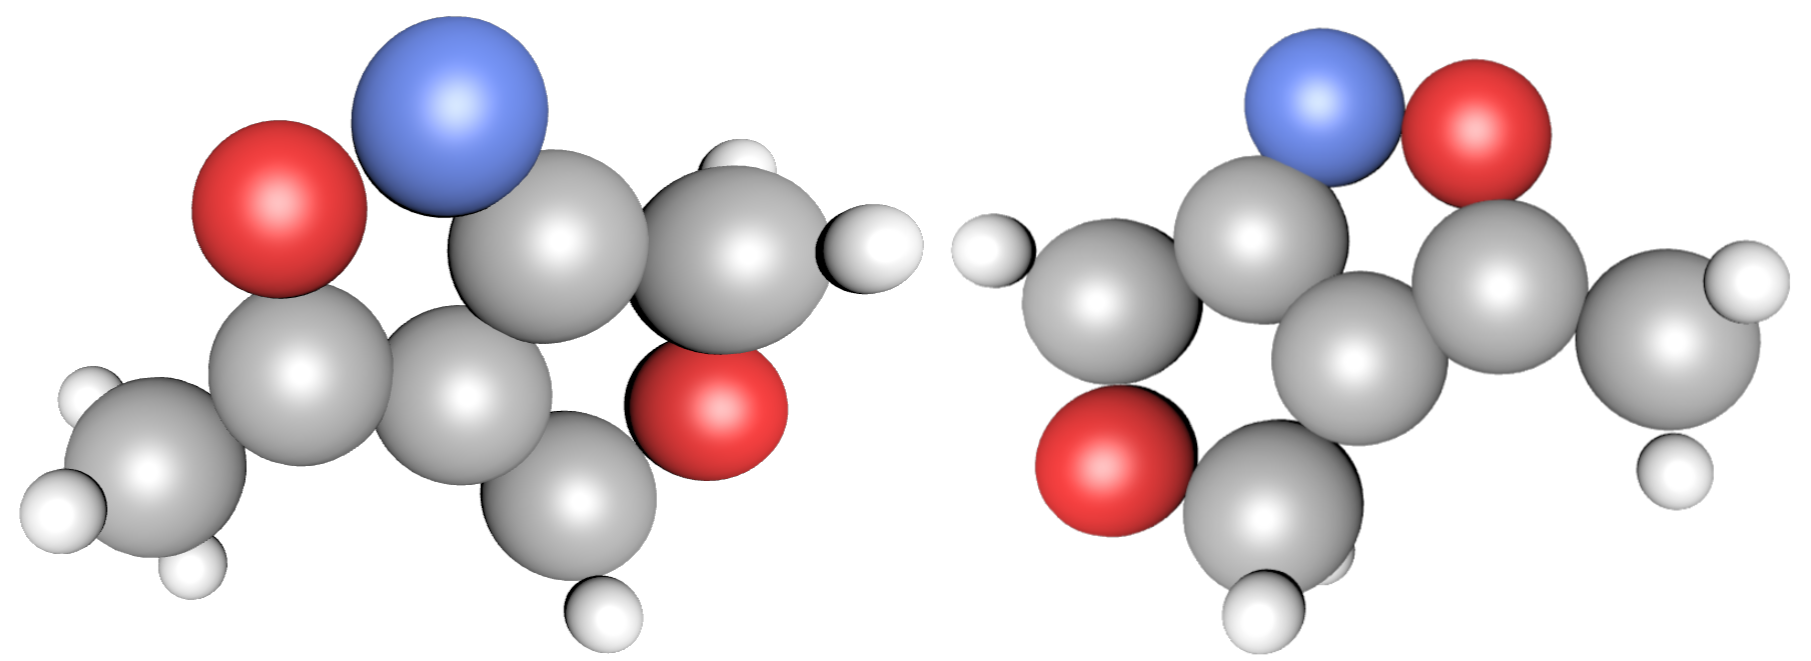
\includegraphics[angle=270, width=\linewidth]{figures/rotation}
	\caption{Two randomly chosen rotations of the same molecule. The values of the atom coordinates are completely different between the two rotations, even though the underlying information is the same.}
	\label{fig:rotation}
\end{figure}

For these reasons, the concrete values of the 3D coordinates, which depend on this arbitrary positioning and rotation of the coordinate system, do not posses relevant information as such. The translation issue could be addressed by instead using directional vectors from one atom to another as edge-features. These vectors are invariant to the arbitrary translation of the molecule in the coordinate system. However, they depend on the arbitrary rotation of the molecule, rendering them also not useful to encode the 3D structure, as shown in the experiment of Section~\ref{sec:direction-vectors}.

In most MPNN architectures, the euclidean distance is provided as an edge feature. This encodes part of the 3D structure in the graph, but still looses vital information. Consider, for instance, the case of the neighborhood of the blue nitrogen atom in Figure~\ref{fig:rotation}. The set of distances to the other atoms is unambiguously derived from the 3D structure (irrespective of the rotation). However, only by knowing the distance to each other atom in the molecule, the structure cannot be derived. There could be a completely different structure giving rise to the same set of distances. For instance, the fact that the blue nitrogen atom is at the margin of the molecule and not in the center is not contained in the information provided by the distances to all other atoms.

%It is straightforward to see that for most graphs with distance as edge feature, there are many 3D structures satisfying these constraints. In other words the mapping from 3D structure to graph with distances is unambiguous but the inverse operation is not.

It does not take much chemical expertise to conjecture that not providing the full 3D structural information to the model limits it's capability to make accurate predictions. However, there is no easy way to avoid this dilemma and, to my knowledge, no satisfying solution has been found so far.

\subsubsection{No down-sampling during feature extraction}

In computer vision with regular CNNs, feature maps are down-sampled to a lower dimension (while expanding the number of channels) every few layers. It makes perfect sense that higher-level features correspond to larger parts of the original image while at the same time requiring more channels to represent the information. Intuitively, one can think of a data-point on a feature map close to the end of the convolutional part as containing features that summarize a larger region of the original image. The connection between higher-level features and lower dimension feature maps is so central to regular CNNs that it is hard to imagine it any other way. However, no analogous process exists in MPNNs (graph convolution).

In MPNNs, the higher-level features (i.e. the node hidden states) are always associated to their respective nodes throughout all message passing steps. While each of the node hidden states contains information from the node's environment, there is no representation that summarizes a whole group of nodes. However, after the graph convolutional layers, all the node representations are immediately aggregated to give a graph representation.

In the case of molecules, such down-sampled representations could represent groups of atoms instead of just individual atoms. In organic chemistry, there are is a limited number of chemical groups, called functional groups, that appear frequently in organic molecules and strongly determine their properties and function. Many of those functional groups are composed of only two to four atoms and appear very frequently in organic molecules (Carbonyl, Hydroxyl, Amide, Amines, etc.)~\cite{Organic-chemistry}. A model with the ability to down-sample would likely learn representations of these important functional groups. Another benefit of such a mechanism would be that it would facilitate the incorporation of angle-information into the model. Note that angles are neither node- nor edge-features. Instead, an angle is a property of a group of three nodes (alternatively, it can also be seen as a property of two edges). Having a representation for a group of - for example three - nodes would allow to add the angle as a feature thus providing more structural information than only distances. For these reasons it is my strong believe that future successful MPNN architectures will likely have some sort of down-sampling mechanism that allows learning representations of groups of nodes.

While no MPNN architecture that reduces the dimensionality of the graph (i.e. groups nodes together) has been found in the literature, some similar approaches have been developed. One of the winning teams of the \textit{Alchemy}-competition~\footnote{\url{https://alchemy.tencent.com/}} found a way to add angles to the message passing framework~\cite{Klicpera2019}. The winning solution in the Kaggle-competition 'Predicting Molecule Properties'~\footnote{\url{https://www.kaggle.com/c/champs-scalar-coupling/discussion/106575}} used atom-triplets and even atom-quadruplets alongside regular atom-nodes in a sort of meta-graph. The result is a very interesting model - however, it proved to be far too large to be trained with the computational resources available for this thesis. Future MPNNs for molecular structures will likely have similar elements to represent features of groups of atoms.

